\chapter{环境化学与毒理学}\label{ch:b3:environmental-toxicology}

每年夏末，卫星都能拍到大湖上蔓延的绿色漩涡：
那是藻类大量繁殖形成的水华，其养料为从农田流失、
又从城镇排出的磷酸盐和硝酸盐。藻类死亡下沉后，分解过程耗尽了
深层水中的氧气，鱼类随之死亡。化学可以解释这条链条的每个环节，以及
许多其他现象：为何某些气体使地球变暖而另一些不会，为何即使空气洁净，雨水仍呈酸性，
农药喷洒之后最终去向何处，以及
某种物质需要多少才会造成危害。本章将平衡、
动力学和光谱学应用于大气、天然水体和土壤，追踪
污染物在它们之间的迁移，最后给出风险评估所依据的
数值。

\begin{recall}
本科一年级分册涵盖酸碱、沉淀和配位平衡、
电势–pH 图、分配系数、半衰期、危害、
风险以及 GHS 体系；第 1 册涵盖\omterm{def:b3:environmental-toxicology:greenhouse}{温室气体}；本科二年级分册涵盖
亨利定律、离子强度、统计学、质谱法和原子
光谱法。\Cref{ch:b3:photochemistry}讨论大气光化学，
\cref{ch:b3:group-theory-applied}和\cref{ch:b3:rovibrational-spectroscopy}讨论\omterm{def:b3:group-theory-applied:activity}{红外活性}，
以及\cref{ch:b3:surfaces-catalysis}讨论\omterm{def:b3:surfaces-catalysis:adsorption}{吸附}。
\end{recall}

\begin{omfigure}
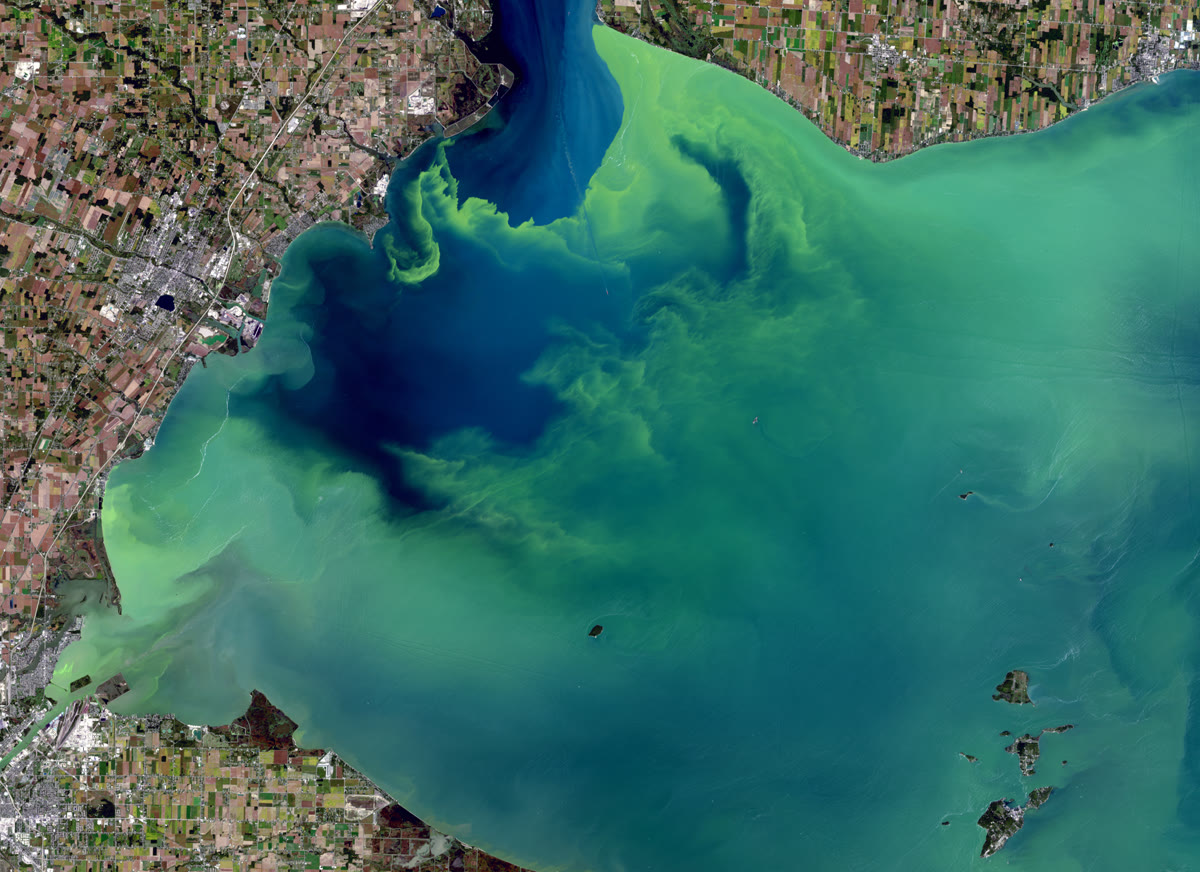
\includegraphics[width=0.62\linewidth]{images/book4/algal-bloom.jpg}

{\small 大湖上的一次藻华，由地球观测卫星在
九月下旬拍摄：绿色漩涡是由微小藻类密集形成的种群，
其养料来自周围农田。图片来源：USGS 和 NASA，公有领域。}
\end{omfigure}

\section{大气层}

\begin{definition}[温室气体]\label{def:b3:environmental-toxicology:greenhouse}
称\emph{温室气体}\index{温室气体}为能够吸收并发射
与地球表面所发射辐射的波长相同的红外辐射，从而使低层大气升温。
气体的\emph{全球变暖
潜能值}\index{全球变暖潜能值}（GWP）是指在某一时间范围（通常为
100 年）内，释放 1 千克该气体后捕获的能量，
与释放 1 千克二氧化碳所捕获能量的比值。
\end{definition}

分子只有通过改变其
偶极矩（见\cref{ch:b3:group-theory-applied}）的振动才能吸收红外辐射。氮气和氧气
均为同核双原子分子，没有这种振动，因此透明；氩气
根本没有振动。二氧化碳为直线形非极性分子，具有\omterm{def:b3:group-theory-applied:activity}{红外活性}的
弯曲振动模式，位于 \qty{15}{\micro\metre} 附近，恰处于地球辐射的中部；水、甲烷
和一氧化二氮则在许多波长处均有吸收。

% ledger: atm:CO2.2025, atm:CH4.2025, atm:N2O.2025, gwp:CH4.fossil, gwp:CH4.nonfossil, gwp:N2O, life:CH4, life:N2O
2025 年全球平均摩尔分数分别为：二氧化碳 \qty{425.6}{ppm}、甲烷 \qty{1936}{ppb} 和
一氧化二氮 \qty{338.9}{ppb}。甲烷可被羟基自由基去除，
寿命约为 12 年，GWP-100 为 27 至 30；一氧化二氮仅在
平流层中被破坏，寿命约为 109 年，GWP-100 为 273。二氧化碳没有
单一寿命：释放出的部分二氧化碳会在空气中留存数百年。

\begin{definition}[空气污染物]\label{def:b3:environmental-toxicology:pollutants}
\emph{颗粒物}\index{颗粒物}是悬浮于空气中的固态和液态
颗粒，按空气动力学直径分类（细颗粒物
直径小于 \qty{2.5}{\micro\metre} 时可深入肺部）。\emph{酸
雨}\index{酸雨}是指酸性强于洁净雨水的雨，
其酸性来自二氧化硫和氮氧化物生成的硫酸和硝酸。
\end{definition}

\begin{proposition}[洁净雨水的 pH]\label{prop:b3:environmental-toxicology:rain-ph}
与今日空气中的二氧化碳达到平衡且别无其他成分的雨水，
pH 约为 5.6。
\end{proposition}

\begin{proof}
% ledger: henry:CO2, pka4:H2CO3.1, pkw4:25C, const:atm
由亨利定律得 $[\ce{CO2(aq)}] = K_Hp(\ce{CO2}) = \qty{3.4e-7}{mol.L^{-1}.Pa^{-1}} \times (425.6 \times 10^{-6} \times \qty{101325}{Pa}) = \qty{1.47e-5}{mol/L}$。
电荷平衡式为 $[\ce{H+}] = [\ce{HCO3-}] + 2[\ce{CO3^2-}] + [\ce{OH-}] \approx K_{a1}[\ce{CO2(aq)}]/[\ce{H+}] + K_w/[\ce{H+}]$，因此
$[\ce{H+}]^2 = K_{a1}[\ce{CO2(aq)}] + K_w = 10^{-6.35} \times \num{1.47e-5} + 10^{-14} = \num{6.6e-12}$：$[\ce{H+}] = \qty{2.6e-6}{mol/L}$，pH 为 5.6。
\end{proof}

含硫燃料燃烧产生的二氧化硫和
高温燃烧产生的氮氧化物，在大气中经羟基自由基和
云滴作用被氧化为硫酸和硝酸，使雨水的 pH 降至 4 甚至更低。
脱除燃料中的硫及尾气中的氮氧化物（催化
转换器、电厂中的氨喷射等）已在应用之处基本解决了
该问题。近地面臭氧由阳光作用于
氮氧化物和挥发性有机化合物而生成（见\cref{ch:b3:photochemistry}），以及
细\omterm{def:b3:environmental-toxicology:pollutants}{颗粒物}，仍是影响健康的主要空气污染物。

\section{天然水体}

\begin{omfigure}
\begin{tikzpicture}
\begin{axis}[name=a, width=0.48\linewidth, height=5.4cm, xmin=4, xmax=13, ymin=0, ymax=1.02,
  axis lines=left, xlabel={pH}, ylabel={溶解碳的分数},
  tick label style={font=\scriptsize}, label style={font=\small}]
\addplot[color=omDef, thick] table[x=pH, y=a0] {figdata/out/bachelor-3-carbonate-system.dat};
\addplot[color=omMeth, thick] table[x=pH, y=a1] {figdata/out/bachelor-3-carbonate-system.dat};
\addplot[color=omThm, thick] table[x=pH, y=a2] {figdata/out/bachelor-3-carbonate-system.dat};
\node[font=\scriptsize, omDef] at (axis cs:4.9,0.85) {$\ce{CO2(aq)}$};
\node[font=\scriptsize, omMeth] at (axis cs:8.3,0.88) {$\ce{HCO3-}$};
\node[font=\scriptsize, omThm] at (axis cs:12.1,0.85) {$\ce{CO3^2-}$};
\draw[black!30, dashed] (axis cs:6.35,0) -- (axis cs:6.35,0.5) (axis cs:10.33,0) -- (axis cs:10.33,0.5);
\end{axis}
\begin{axis}[at={(a.east)}, anchor=west, xshift=1.4cm, width=0.48\linewidth, height=5.4cm,
  xmin=0, xmax=2000, ymin=5.2, ymax=6.2, axis lines=left,
  xlabel={空气中 $\ce{CO2}$ / ppm}, ylabel={雨水的 pH},
  tick label style={font=\scriptsize}, label style={font=\small},
  scaled x ticks=false, xticklabel style={/pgf/number format/1000 sep={}}]
\addplot[color=omDef, thick] table[x=ppm, y=pH] {figdata/out/bachelor-3-carbonate-system-b.dat};
\draw[black!35, dashed] (axis cs:425.6,5.2) -- (axis cs:425.6,5.59);
\node[font=\scriptsize, anchor=west] at (axis cs:470,5.63) {今日：5.6};
\end{axis}
\end{tikzpicture}

{\small 左图：溶解无机碳三种形态的分布
随 pH 变化（\qty{25}{\celsius}），两曲线交于 $\mathrm pK_{a1} = 6.35$ 和 $\mathrm pK_{a2} = 10.33$。右图：仅与二氧化碳平衡的雨水
pH 随其在空气中的摩尔分数而变化。}
\end{omfigure}

\begin{proposition}[碳酸盐的组分分数]\label{prop:b3:environmental-toxicology:carbonate-fractions}
设 $C_T$ 为溶解无机碳的总量，
$[\ce{CO2(aq)}] = C_Th^2/D$，$[\ce{HCO3-}] = C_TK_{a1}h/D$，$[\ce{CO3^2-}] = C_TK_{a1}K_{a2}/D$，其中 $h = [\ce{H+}]$，$D = h^2 + K_{a1}h + K_{a1}K_{a2}$。
\end{proposition}

\begin{proof}
由两个酸度常数，
\[
  [\ce{HCO3-}] = \frac{K_{a1}[\ce{CO2(aq)}]}{h}, \qquad [\ce{CO3^2-}] = \frac{K_{a2}[\ce{HCO3-}]}{h} = \frac{K_{a1}K_{a2}[\ce{CO2(aq)}]}{h^2}.
\]
三者之和为 $C_T = [\ce{CO2(aq)}]\,D/h^2$；将各形态除以 $C_T$ 即得其分数。
\end{proof}

\begin{definition}[碱度]\label{def:b3:environmental-toxicology:alkalinity}
水的\emph{碱度}\index{碱度}是指其
中和强酸的能力，以滴定至碳酸的滴定终点（约 pH
4.5）测定，并以每升所含 $\ce{H+}$ 的摩尔数表示。
\end{definition}

\begin{proposition}[碳酸盐碱度]\label{prop:b3:environmental-toxicology:alkalinity}
在碱性成分为碳酸盐类与氢氧根的水中，
$\mathrm{Alk} = [\ce{HCO3-}] + 2[\ce{CO3^2-}] + [\ce{OH-}] - [\ce{H+}]$；其值等于强碱阳离子所带的电荷
超出强酸阴离子所带电荷的部分，且二氧化碳
与空气交换时不随之改变。
\end{proposition}

\begin{proof}
滴定至碳酸的终点时，每个 $\ce{HCO3-}$ 转化为 $\ce{CO2}$（各消耗一个 $\ce{H+}$），
每个 $\ce{CO3^2-}$ 转化为 $\ce{CO2}$（消耗两个），每个 $\ce{OH-}$ 转化为水（消耗一个），而原有的游离 $\ce{H+}$
起相反作用，即得上述和式。水的电荷平衡中含有
$\ce{Na+}$、$\ce{Ca^2+}$\dots{} 与 $\ce{Cl-}$、$\ce{SO4^2-}$\dots 的电荷平衡式，经整理后得同一和式，即强电解质的 $\sum z_i c_i$（阳离子）$-$ $\sum z_jc_j$（阴离子）
之差。加入或移除 $\ce{CO2}$ 不改变其中任何离子。
\end{proof}

\begin{definition}[海洋酸化]\label{def:b3:environmental-toxicology:acidification}
\emph{海洋酸化}\index{海洋酸化}是指海水吸收空气中的
二氧化碳时 pH 的降低。碳酸盐矿物的\emph{饱和度}\index{饱和度}
定义为
$\Omega = [\ce{Ca^2+}][\ce{CO3^2-}]/K_{sp}$：大于 1 时矿物可以形成，小于 1 时则趋于溶解。
\end{definition}

溶解的二氧化碳使碳酸根离子转化为碳酸氢根，$\ce{CO2 + CO3^2- + H2O -> 2HCO3-}$，
使 pH 和 $\Omega$ 降低，贝壳与珊瑚骨骼更难形成。（在
海水中，常数为表观常数，在盐介质中测得，
与本章中淡水的数值不同。）

\begin{definition}[水的硬度]\label{def:b3:environmental-toxicology:hardness}
水的\emph{硬度}\index{硬度}是指其
钙离子与镁离子的总浓度，通常以
含有相同摩尔数的碳酸钙质量表示，单位为 mg/L。
\end{definition}

\begin{definition}[需氧量]\label{def:b3:environmental-toxicology:oxygen-demand}
水的\emph{生化需氧量}\index{生化需氧量}（BOD）是指
每升水中的有机物被微生物在黑暗中氧化时所消耗的氧气质量，
在规定时间内（\qty{20}{\celsius} 下的五天，即 $\mathrm{BOD_5}$）。其
\emph{化学需氧量}\index{化学需氧量}（COD）是指
与化学氧化其有机物时所消耗重铬酸盐相当的
氧气质量。
\end{definition}

\begin{proposition}[BOD 曲线]\label{prop:b3:environmental-toxicology:bod}
若可生物降解的有机物按一级动力学被消耗，速率
常数为 $k$，则经过时间 $t$ 后所消耗的氧量为 $\mathrm{BOD}_t = L_0(1 - \eu^{-kt})$，其中 $L_0$ 为最终 BOD。
\end{proposition}

\begin{proof}
剩余需氧量 $L$ 满足 $\dd L/\dd t = -kL$，故 $L = L_0\eu^{-kt}$；所消耗的氧量即已减少的量，
即 $L_0 - L$。
\end{proof}

\begin{omfigure}
\begin{tikzpicture}
\begin{axis}[name=a, width=0.48\linewidth, height=5.2cm, xmin=0, xmax=30, ymin=0, ymax=270,
  axis lines=left, xlabel={时间 / 天}, ylabel={BOD / \unit{mg.L^{-1}}},
  tick label style={font=\scriptsize}, label style={font=\small}]
\addplot[color=omDef, thick] table[x=t, y=bod] {figdata/out/bachelor-3-bod.dat};
\draw[black!35, dashed] (axis cs:0,250) -- (axis cs:30,250);
\draw[black!35, dashed] (axis cs:5,0) -- (axis cs:5,170.8);
\node[font=\scriptsize, anchor=west] at (axis cs:5.6,140) {$\mathrm{BOD_5}$};
\node[font=\scriptsize, anchor=north east] at (axis cs:30,246) {$L_0$};
\end{axis}
\begin{axis}[at={(a.east)}, anchor=west, xshift=1.4cm, width=0.48\linewidth, height=5.2cm,
  xmin=0, xmax=15, ymin=0, ymax=10, axis lines=left,
  xlabel={下游时间 / 天}, ylabel={溶解的 $\ce{O2}$ / \unit{mg.L^{-1}}},
  tick label style={font=\scriptsize}, label style={font=\small}]
\addplot[color=omThm, thick] table[x=t, y=O2] {figdata/out/bachelor-3-bod-b.dat};
\draw[black!35, dashed] (axis cs:0,9.1) -- (axis cs:15,9.1);
\node[font=\scriptsize, anchor=south east] at (axis cs:15,9.1) {饱和};
\node[font=\scriptsize, anchor=north] at (axis cs:2.4,6.3) {临界点};
\end{axis}
\end{tikzpicture}

{\small 左图：某模型污水的 BOD，$L_0 = \qty{250}{mg/L}$，$k = \qty{0.23}{d^{-1}}$：约三分之二的
需氧量在五天内被消耗。右图：排污口下游河流中的氧垂
（斯特里特–费尔普斯模型）：有机负荷分解消耗氧气，其速度快于
空气起初的复氧速度，直至亏氧量在约 2.4 天时达到峰值。}
\end{omfigure}

\begin{method}[化学需氧量的测定]\label{met:b3:environmental-toxicology:cod}
\begin{enumerate}
  \item 取一定体积的水样，在加热回流条件下与已知过量的重铬酸钾
        的硫酸溶液反应，以硫酸银为催化剂，
        以硫酸汞（II）络合氯离子。
  \item 以邻菲罗啉亚铁为指示剂，用亚铁（II）盐滴定剩余的重铬酸盐，并
        以纯水代替水样做空白实验。
  \item 所消耗的重铬酸盐，换算成相当的 $\ce{O2}$ 质量（一个
        $\ce{Cr2O7^2-}$ 得六个电子，相当于 1.5 $\ce{O2}$），除以水样体积后，即为
        \omterm{def:b3:environmental-toxicology:oxygen-demand}{化学需氧量}，单位为 mg/L。
\end{enumerate}
\end{method}

\begin{definition}[富营养化]\label{def:b3:environmental-toxicology:eutrophication}
称\emph{富营养化}\index{富营养化}为水体富集了营养物质（主要是磷和氮），
导致藻类和水生植物过度生长，
随后藻类和植物死亡分解，又使水中溶解氧耗尽。
\end{definition}

\begin{omfigure}
\begin{tikzpicture}[font=\scriptsize, >=Stealth,
  box/.style={draw, rounded corners, align=center, fill=omMeth!10, inner sep=3pt, minimum height=8mm}]
  \node[box] (f) at (-3.4,1.2) {田地：化肥、\\ 粪肥};
  \node[box] (t) at (-3.4,-0.4) {城镇：污水、\\ 洗涤剂};
  \node[box] (a) at (0,2.1) {大气：\\ 沉降（N）};
  \node[box, fill=omDef!12, minimum width=3.2cm, minimum height=1.7cm] (l) at (0.6,0.4) {湖水：\\ 藻类生长};
  \node[box, fill=black!8] (s) at (0.6,-1.6) {沉积物：储存 P，\\ 缺氧时释放};
  \node[box] (o) at (4.0,0.4) {流出};
  \draw[->, thick] (f) -- node[above, sloped, pos=0.4] {径流} (l);
  \draw[->, thick] (t) -- node[below, sloped] {N、P} (l);
  \draw[->, thick] (a) -- (l);
  \draw[->, thick] (l) -- node[left] {死亡藻类} (s);
  \draw[->, thick, dashed] (s.east) to[bend right=30] node[right] {P} (l.south east);
  \draw[->, thick] (l) -- (o);
\end{tikzpicture}

{\small 营养物质流入湖泊并在湖中迁移。磷通常是淡水中的限制性营养物质，
在沉积物中累积，底层缺氧时又回到水中，
这使水华在营养输入
被切断后仍可持续数年。}
\end{omfigure}

藻类摄取碳、氮、磷的比例大致恒定；
相对于这些需求而言短缺的营养元素会限制藻类的生长。
大多数湖泊中限制因素是磷，这也是磷酸盐被从
洗涤剂和经处理的污水中去除的原因；许多近海海域中则是氮。

\begin{definition}[化学形态]\label{def:b3:environmental-toxicology:speciation}
称样品中某元素的\emph{化学形态}\index{化学形态}为
其物质的量在各化学形态间的分配情况，
这些形态包括：氧化态、配合物、有机金属化合物，以及游离态和结合态物种。
\end{definition}

毒性取决于形态。释放到水中的无机汞
会被沉积物中的细菌甲基化为甲基汞，甲基汞能穿过膜，
与蛋白质中的硫结合，并沿食物链富集；砷以亚砷酸根 As(III) 存在时的
毒性远大于以砷酸根 As(V) 存在时，而海产品中所含有机形态的
毒性则小得多。仅凭总浓度难以说明问题。

\begin{method}[水体中金属的化学形态分析]\label{met:b3:environmental-toxicology:speciation}
\begin{enumerate}
  \item 列出存在的配体（氢氧根、碳酸根、氯离子、硫酸根、有机
        物）及其浓度和 pH。
  \item 写出配合常数与金属的质量守恒式，
        如本科一年级分册中所述。
  \item 求出游离金属离子，再逐一求出各配合物；
        作出各形态分数随 pH 或配体浓度变化的图。
  \item 将有毒或可生物利用的形态（通常为游离离子）与总浓度进行比较。
\end{enumerate}
\end{method}

\section{土壤与沉积物}

\begin{definition}[土壤中的吸附]\label{def:b3:environmental-toxicology:soil}
称土壤的\emph{阳离子交换容量}\index{阳离子交换容量}为
单位质量土壤所能保持的可交换阳离子的量，这些阳离子
\omterm{def:b3:surfaces-catalysis:adsorption}{吸附}于黏土和有机质上。\emph{土–水分配系数}\index{土–水分配系数}
$K_d$ 为\omterm{def:b3:surfaces-catalysis:adsorption}{吸附}在土壤上的某物质浓度（每千克）
与其在孔隙水中浓度（每升）之比；
\emph{有机碳分配系数}\index{有机碳分配系数}为
$K_{oc} = K_d/f_{oc}$，其中 $f_{oc}$ 为有机碳的质量分数。
\end{definition}

中性有机化合物主要\omterm{def:b3:surfaces-catalysis:adsorption}{吸附}在土壤有机质上，因此 $K_{oc}$ 随土壤不同而
变化远小于 $K_d$。$K_d$ 较小的化合物随水迁移，
可能到达地下水（淋溶）；$K_d$ 较大的化合物则留在表层附近，
与颗粒结合，这些颗粒可能被侵蚀带入河流和湖泊。

\section{污染物的归宿}

\begin{definition}[辛醇–水分配系数]\label{def:b3:environmental-toxicology:kow}
称某物质的\emph{辛醇–水分配系数}\index{辛醇–水分配系数}
$K_{ow}$ 为其在辛-1-醇和水中的平衡浓度之比，
它表征该物质对脂肪组织和有机
物的亲和力。
\end{definition}

% ledger: logkow:DDT, logkow:benzene, logkow:atrazine, logkow:PCB153
苯的 $\log K_{ow} = 2.13$，除草剂阿特拉津为 2.61，六氯代多氯联苯为 6.67，
滴滴涕为 6.91：后两者在脂肪中的溶解度
比在水中高出数千万倍。

\begin{definition}[生物累积]\label{def:b3:environmental-toxicology:bio}
称\emph{生物富集系数}\index{生物富集系数}（BCF）为
稳态时生物体内浓度与周围水中浓度之比，
仅考虑从水中摄取的情况。\emph{生物累积}\index{生物累积}
指生物体经所有途径（包括食物）积累某物质的过程；
\emph{生物放大}\index{生物放大}指
沿食物链由猎物到捕食者浓度逐级升高的现象。
\end{definition}

\begin{proposition}[BCF 与 $K_{ow}$]\label{prop:b3:environmental-toxicology:bcf-kow}
对于不被代谢的中性有机物，鱼体内 $\log\mathrm{BCF}$ 近似为
$\log K_{ow}$ 的线性函数，斜率接近 1，直到 $\log K_{ow}$ 约为 6；
超过此值后，摄取速率变慢，关系趋于平缓（经验回归）。
\admitted
\end{proposition}

\begin{definition}[持久性有机污染物]\label{def:b3:environmental-toxicology:pop}
称\emph{持久性有机污染物}\index{持久性有机污染物}为
一类有机物质，它抗降解、可\omterm{def:b3:environmental-toxicology:bio}{生物累积}、有毒性，并
可远距离输送，例如滴滴涕、多氯联苯和二恶英。
\end{definition}

\begin{proposition}[平衡状态下各相之间的分配]\label{prop:b3:environmental-toxicology:level-one}
质量为 $M$ 的物质在平衡状态下（“一级”模型）分配于水
（体积 $V_w$）、空气（$V_a$）、沉积物固体（$m_s$）和鱼（$m_f$）之中，其水中浓度为
$C_w = M/(V_w + K_{aw}V_a + K_{sw}m_s + K_{fw}m_f)$，其中 $K$ 为相对于水的分配系数；
每一相中的质量等于该相的对应项乘以 $C_w$。
\end{proposition}

\begin{proof}
平衡时 $C_a = K_{aw}C_w$，$C_s = K_{sw}C_w$（按每千克计），$C_f = K_{fw}C_w$。质量守恒给出
$M = C_wV_w + C_aV_a + C_sm_s + C_fm_f = C_w(V_w + K_{aw}V_a + K_{sw}m_s + K_{fw}m_f)$；两边除以括号内之和即得 $C_w$。
\end{proof}

\begin{omfigure}
\begin{tikzpicture}[font=\scriptsize, >=Stealth,
  comp/.style={draw, rounded corners, align=center, minimum width=2.6cm, minimum height=1.0cm}]
  \node[comp, fill=omDef!8] (air) at (0,2.2) {空气 \\ $C_a = K_{aw}C_w$};
  \node[comp, fill=omDef!25] (w) at (0,0.6) {水 \\ $C_w$};
  \node[comp, fill=black!10] (sed) at (0,-1.0) {沉积物 \\ $C_s = K_{sw}C_w$};
  \node[comp, fill=omMeth!15] (fish) at (3.6,0.6) {鱼 \\ $C_f = K_{fw}C_w$};
  \node[comp, fill=omProp!15] (soil) at (-3.6,0.6) {土壤 \\ $C_{\text{土壤}} = K_dC_w$};
  \draw[<->, thick] (air) -- (w); \draw[<->, thick] (w) -- (sed);
  \draw[<->, thick] (w) -- (fish); \draw[<->, thick] (w) -- (soil);
\end{tikzpicture}

{\small 平衡（一级）模型的各相：每一相都与水处于平衡，
其浓度由分配系数确定。
物质在容量与体积（或质量）之积最大的相中积累，
对于疏水性化合物，通常是沉积物或土壤。}
\end{omfigure}

\section{毒理学与法规}

\begin{definition}[剂量–效应]\label{def:b3:environmental-toxicology:dose}
称\emph{剂量–效应关系}\index{剂量–效应关系}为
物质的剂量与效应的大小或频率之间的联系。\emph{半数致死量}\index{半数致死量}
$\mathrm{LD_{50}}$ 可致死一半的受试群体；
\emph{半数效应浓度}\index{半数效应浓度} $\mathrm{EC_{50}}$ 使一半个体产生规定的效应。
\emph{未观察到有害作用剂量}\index{未观察到有害作用剂量}
（NOAEL）是未出现有害效应的最高受试剂量，
\emph{最低观察到有害作用剂量}\index{最低观察到有害作用剂量}
（LOAEL）则是
出现有害效应的最低受试剂量。
\end{definition}

\begin{proposition}[对数–逻辑斯谛模型]\label{prop:b3:environmental-toxicology:dose-response}
在对数–逻辑斯谛模型 $f(d) = 1/\bigl(1 + (D_{50}/d)^n\bigr)$ 中，当 $d = D_{50}$ 时响应为一半，$n$
刻画曲线的陡峭程度：10\,\% 与 90\,\% 响应对应的剂量之比为 $81^{1/n}$。
\end{proposition}

\begin{proof}
当 $d = D_{50}$ 时，$f = 1/2$。$f = 0.1$ 要求 $(D_{50}/d)^n = 9$，$f = 0.9$ 要求 $(D_{50}/d)^n = 1/9$；两剂量之比为
$(9 \times 9)^{1/n} = 81^{1/n}$。
\end{proof}

\begin{omfigure}
\begin{tikzpicture}
\begin{axis}[width=0.72\linewidth, height=5.4cm, xmode=log, xmin=3, xmax=3200, ymin=0, ymax=1.02,
  axis lines=left, xlabel={剂量 / \unit{mg.kg^{-1}}}, ylabel={响应比例},
  tick label style={font=\scriptsize}, label style={font=\small}]
\addplot[color=omDef, thick] table[x=d, y=n2] {figdata/out/bachelor-3-dose-response.dat};
\addplot[color=omThm, thick] table[x=d, y=n6] {figdata/out/bachelor-3-dose-response.dat};
\addplot[only marks, mark=*, mark size=1.6pt, omThm] table[x=d, y=r] {figdata/out/bachelor-3-dose-response-b.dat};
\draw[black!35, dashed] (axis cs:200,0) -- (axis cs:200,0.5) -- (axis cs:3,0.5);
\node[font=\scriptsize, anchor=north west] at (axis cs:200,0.48) {$D_{50}$};
\node[font=\scriptsize, omThm, anchor=south east, inner sep=1pt] (noael) at (axis cs:60,0.09) {NOAEL};
\draw[omThm] (noael.south east) -- (axis cs:78,0.012);
\node[font=\scriptsize, omThm, anchor=west] at (axis cs:165,0.2) {LOAEL};
\node[font=\scriptsize, omDef, anchor=east] at (axis cs:60,0.25) {$n = 2$};
\node[font=\scriptsize, omThm, anchor=east] at (axis cs:185,0.8) {$n = 6$};
\end{axis}
\end{tikzpicture}

{\small 对数–逻辑斯谛剂量–响应曲线，相同中位剂量（\qty{200}{mg/kg}，
模型）、两种陡峭程度。圆点为较陡曲线在五个剂量下的一项研究：
以 5\,\% 响应作为有害效应的判据，NOAEL 为
\qty{80}{mg/kg}，LOAEL 为 \qty{160}{mg/kg}；两者都取决于所选的剂量。}
\end{omfigure}

\begin{definition}[急性毒性与慢性毒性]\label{def:b3:environmental-toxicology:toxicity}
\emph{急性毒性}\index{急性毒性}是指一次接触或在短时间内多次接触所造成的危害；
\emph{慢性毒性}\index{慢性毒性}则是指
在生命的较长部分内反复或持续接触所造成的危害。
\end{definition}

% ledger: ld50:NaCl, ld50:caffeine, ld50:nicotine
毒性取决于剂量：在大鼠中，氯化钠经口的 $\mathrm{LD_{50}}$ 约为 \qty{3000}{mg/kg}，
同类记录中咖啡因为 \qty{192}{mg/kg}，尼古丁为 \qty{188}{mg/kg}。对于多数效应，
存在阈剂量，低于该剂量时机体可以应对；对于遗传毒性致癌物，
则不假定存在阈值，接触量应保持在合理可行的尽可能低的水平。

\begin{definition}[生态毒理学]\label{def:b3:environmental-toxicology:ecotoxicology}
\emph{生态毒理学}\index{生态毒理学}研究物质对
生态系统中生物体的影响。\emph{预测无效应浓度}\index{预测无效应浓度}
（PNEC）是对代表性物种进行试验所得的最低
效应浓度或无效应浓度，
再除以用于涵盖不确定度的评估因子；\emph{预测环境浓度}\index{预测环境浓度}
（PEC）是由该物质的用途和归宿所预期的浓度；
\emph{风险商}\index{风险商}为
PEC/PNEC。
\end{definition}

\begin{proposition}[风险商]\label{prop:b3:environmental-toxicology:risk-quotient}
\omterm{def:b3:environmental-toxicology:ecotoxicology}{风险商}小于 1 表明所评估的相中无须关注；
大于 1 则为一种风险，需要更精确的数据或采取措施降低接触。
\end{proposition}

\begin{proof}[由定义可得]
PNEC 通过其评估因子被设定在观察到效应的各浓度之下；
因此，预期浓度低于它时不预期产生效应，
高于它时则预期产生效应。
\end{proof}

\begin{method}[环境风险评估]\label{met:b3:environmental-toxicology:risk}
\begin{enumerate}
  \item 危害：收集藻类、无脊椎动物和鱼类的毒性数据（急性
        $\mathrm{EC_{50}}$、慢性 NOEC）；取其中最低值，再除以评估因子（仅有急性数据时
        取较大的因子），得到 PNEC。
  \item 暴露：依据使用量及归宿（分配、降解），
        计算各相中的 PEC，或直接测量。
  \item 风险：计算 PEC/PNEC；若大于 1，则
        完善数据或减少接触，并重复上述步骤。
\end{enumerate}
\end{method}

\begin{definition}[职业接触限值]\label{def:b3:environmental-toxicology:oel}
\emph{职业接触限值}\index{职业接触限值}是指
工作场所空气中某物质的浓度，工人在此浓度下可以呼吸，
按一个工作日平均（短期限值按 15 分钟平均），且
不预期产生有害效应。
\end{definition}

大量投放市场的新化学品必须登记，
并提交一份关于其性质、危害和用途的档案；危害最大者可能受到限制，
或仅允许用于经批准的用途。

\begin{inthelab}[测定 $\mathrm{BOD_5}$]
将样品用含营养物的曝气稀释水稀释，并加入细菌菌种，
使氧气被消耗一大部分，但不全部耗尽。取两个磨口瓶装满至溢出，
其中一瓶的溶解氧立即用氧电极测定，
另一瓶在黑暗中于 \qty{20}{\celsius} 放置五天后再测定。
两者之差乘以稀释倍数，并扣除菌种的影响，即为
$\mathrm{BOD_5}$。
\end{inthelab}

\begin{safety}{\ghs[0.62cm]{GHS03}\ghs[0.62cm]{GHS05}\ghs[0.62cm]{GHS06}\ghs[0.62cm]{GHS08}\ghs[0.62cm]{GHS09}}
% ledger: ghs:K2Cr2O7, ghs4:HgSO4
COD 试剂：重铬酸钾是氧化剂，可能致癌并引起遗传缺陷，
具有腐蚀性和致敏性；硫酸汞吞食、吸入或与皮肤接触时均会致命，
并且对水生生物毒性很大。两者都用于密封试管中，
用过的试管应作为危险废物处理。
\end{safety}

\begin{history}[一本书与一个海湾]
1962 年，蕾切尔·卡森的 《寂静的春天》 描述了鸟类因
DDT 及其他农药沿食物链富集而中毒、数量下降，并推动了现代
环境法规的建立。数年前的 1956 年，水俣湾的居民中
出现了一种神经系统疾病：一家化工厂排放了甲基汞，
该甲基汞由其所用的汞催化剂生成，
并在居民所食用的鱼体内积累。
\end{history}

\section{练习}

\begin{exercise}[$\star$]\label{exo:b3:environmental-toxicology:1}
为什么 $\ce{N2}$、$\ce{O2}$ 和 Ar 不吸收红外线，$\ce{CO2}$ 的哪种振动使其成为
\omterm{def:b3:environmental-toxicology:greenhouse}{温室气体}？
\end{exercise}

\begin{exercise}[$\star$]\label{exo:b3:environmental-toxicology:2}
当海水的 pH 下降 0.1 时，$[\ce{H+}]$ 变为原来的多少倍？
\end{exercise}

\begin{exercise}[$\star$]\label{exo:b3:environmental-toxicology:3}
某水样中含 \qty{2.0}{mmol/L} 的 $\ce{Ca^2+}$ 和 \qty{0.50}{mmol/L} 的 $\ce{Mg^2+}$。求其\omterm{def:b3:environmental-toxicology:hardness}{硬度}，以每升水中所含 $\ce{CaCO3}$ 的毫克数表示。
\end{exercise}

\begin{exercise}[$\star$]\label{exo:b3:environmental-toxicology:4}
藻类摄取 C、N 和 P 的摩尔比为 $106 : 16 : 1$（练习数据）。某湖水中含有
\qty{0.60}{mg/L} 的硝酸盐氮和 \qty{0.010}{mg/L} 的磷酸盐磷；哪种营养物限制了
生长？
\end{exercise}

\begin{exercise}[$\star\star$]\label{exo:b3:environmental-toxicology:5}
对某污水测得 $\mathrm{BOD_5}$ 为 \qty{170}{mg/L}，其 $k = \qty{0.23}{d^{-1}}$。估算其最终\omterm{def:b3:environmental-toxicology:oxygen-demand}{生化需氧量}。
\end{exercise}

\begin{exercise}[$\star\star$]\label{exo:b3:environmental-toxicology:6}
取 \qty{100.0}{mL} 水样，需加入 \qty{4.40}{mL} 浓度为 \qty{0.0200}{mol/L} 的盐酸才能使其 pH 达到 4.5。计算其
\omterm{def:b3:environmental-toxicology:alkalinity}{碱度}；并假设\omterm{def:b3:environmental-toxicology:alkalinity}{碱度}全部来自碳酸氢根，求其以 mg/L 表示的浓度。
\end{exercise}

\begin{exercise}[$\star\star$]\label{exo:b3:environmental-toxicology:7}
某土壤的 $f_{oc} = 0.020$；某农药的 $K_{oc} = \qty{300}{L/kg}$（练习数据）。计算 $K_d$ 以及
以 \qty{1.5}{kg} 固体对应 \qty{0.30}{L} 孔隙水的土壤中，被\omterm{def:b3:surfaces-catalysis:adsorption}{吸附}的农药所占比例。
\end{exercise}

\begin{exercise}[$\star\star$]\label{exo:b3:environmental-toxicology:8}
取经验回归式 $\log\mathrm{BCF} = 0.85\log K_{ow} - 0.70$（练习数据），估算
苯及一种六氯代多氯联苯的 BCF，并加以评论。
\end{exercise}

\begin{exercise}[$\star\star$]\label{exo:b3:environmental-toxicology:9}
将大鼠经口咖啡因的 $\mathrm{LD_{50}}$ 换算为一位 \qty{70}{kg} 成年人的质量，并换算为咖啡杯数，每杯含
\qty{90}{mg} 咖啡因（粗略换算，练习数据）。为什么这种换算只具有参考意义？
\end{exercise}

\begin{exercise}[$\star\star\star$]\label{exo:b3:environmental-toxicology:10}
某物质的 48 小时 $\mathrm{EC_{50}}$（水蚤）为 \qty{0.50}{mg/L}，72 小时 $\mathrm{EC_{50}}$（藻类）为 \qty{1.2}{mg/L}，
96 小时 $\mathrm{LC_{50}}$（鱼类）为 \qty{2.0}{mg/L}，均为急性数据，并适用评估因子 1000
（练习数据）。计算 PNEC，以及 PEC 为 \qty{0.20}{\micro g/L} 时的\omterm{def:b3:environmental-toxicology:ecotoxicology}{风险商}。
\end{exercise}

\begin{exercise}[$\star\star\star$]\label{exo:b3:environmental-toxicology:11}
某食鱼鸟类所食的鱼中含有 \qty{0.30}{mg/kg} 的持久性污染物；鱼所食的
浮游生物含有 \qty{0.015}{mg/kg}；水中含有 \qty{2.0}{ng/L}。计算沿食物链的\omterm{def:b3:environmental-toxicology:bio}{生物富集
系数}和\omterm{def:b3:environmental-toxicology:bio}{生物放大}系数，若鸟类脂肪中含 \qty{6.0}{mg/kg}（练习
数据）。
\end{exercise}

\begin{exercise}[$\star\star\star$]\label{exo:b3:environmental-toxicology:12}
某电厂每年排放 \qty{1000}{t} 的 $\ce{SO2}$。计算其能够生产的硫酸质量，
以及全部排放物都随雨降下时，使雨水 pH 降至 4.0 所对应的雨水体积（忽略其他
酸和碱的影响）。
\end{exercise}

\section{问题：湖中的一种农药}

\begin{problem}[{周末问题——湖中的一种农药：它在沉积物和鱼体中的分配，
平衡态质量衡算，其一年内的降解，
以及湖泊生物的风险商}]
\label{pb:b3:environmental-toxicology:1}
题目数据。某湖泊含水 $\qty{1.0e9}{L}$，其上方（混合层）空气为 $\qty{1.0e12}{L}$，
并含活性沉积物固体 $\qty{1.0e8}{kg}$（$f_{oc} = 0.040$）和鱼 $\qty{1.0e4}{kg}$（脂质分数 0.048）。
某农药 $\log K_{ow} = 4.0$，空气–水分配系数 $K_{aw} = \num{1.0e-4}$，且 $K_{oc} = 0.41\,K_{ow}$；
$K_{fw}$ = 脂质分数 $\times K_{ow}$。共 100 千克该农药进入湖中，其在湖中的半衰期为 60 天。
最敏感的慢性试验给出 NOEC 为 \qty{50}{\micro g/L}，评估因子取 10；
供人食用的鱼体中该农药含量不应超过 \qty{1.0}{mg/kg}。

\medskip\noindent\textbf{第一部分——分配系数。}
\begin{enumerate}
  \item 数据 $\log K_{ow} = 4.0$ 说明该农药具有什么性质？
  \item 计算 $K_{oc}$ 及沉积物–水分配系数 $K_{sw}$。
  \item 计算鱼–水分配系数 $K_{fw}$。
  \item 该农药是否容易从水中挥发？利用 $K_{aw}$ 判断。
  \item 为何\omterm{def:b3:surfaces-catalysis:adsorption}{吸附}主要受有机碳控制，而非矿物质？
  \item 你认为哪一个相中积累的该农药最多？
\end{enumerate}

\medskip\noindent\textbf{第二部分——平衡态质量衡算。}
\begin{enumerate}[resume]
  \item 计算容量项 $V_w$、$K_{aw}V_a$、$K_{sw}m_s$ 和 $K_{fw}m_f$。
  \item 计算水相浓度。
  \item 计算各相中的质量。
  \item 计算空气、沉积物和鱼中的浓度。
  \item 模型中哪一个假设最不符合实际？
  \item 考虑降解后（II 级和 III 级模型），结果会如何变化？
\end{enumerate}

\medskip\noindent\textbf{第三部分——降解。}
\begin{enumerate}[resume]
  \item 计算一级速率常数。
  \item 计算一年后剩余的分数。
  \item 计算一年后水相浓度。
  \item 为何沉积物中的该农药可能比半衰期所暗示的时间保留更久？
  \item 什么因素使农药具有持久性？
\end{enumerate}

\medskip\noindent\textbf{第四部分——风险。}
\begin{enumerate}[resume]
  \item 计算 PNEC。
  \item 取初始水相浓度作为 PEC，计算\omterm{def:b3:environmental-toxicology:ecotoxicology}{风险商}。
  \item 就湖泊生物给出结论。
  \item 将鱼体中的浓度与食用限值进行比较。
  \item 接下来应测量什么，在何处测量？
  \item 哪些措施可以降低 PEC？
  \item 为何评估因子如此重要？
  \item 给出结果：\omterm{def:b3:environmental-toxicology:ecotoxicology}{风险商} PEC/PNEC。
\end{enumerate}
\end{problem}
